\documentclass{article}
\usepackage{natbib}
\usepackage[labelfont=bf]{caption}
\usepackage{subcaption}
\usepackage{graphicx}
\usepackage{float}
\bibliographystyle{apalike}
\usepackage{lineno}
\linenumbers

\usepackage{geometry}
\geometry{letterpaper}
\geometry{margin=1in}

\usepackage{setspace}
\doublespacing
\captionsetup[figure]{font={stretch=2}}

\usepackage{authblk}
\usepackage{xcolor}

\newcommand{\matr}[1]{\mathbf{#1}}

%\title{Improving Accuracy of Simulated Flows in Steeply Dipping Layers Using full connectivity Grids with the XT3D Multi-Point Flux Approximation in MODFLOW 6}

% suggested title revision
\title{Efficient and Accurate Modeling of Flow through Sedimentary Structures with MODFLOW 6}

\author{
	Alden M. Provost, U.S. Geological Survey, Integrated Modeling and Prediction Division, U.S. Geological Survey, 12201 Sunrise Valley Dr, Reston, VA, USA  \\
	\and 
	Kerry Bardot, School of Earth Sciences, University of Western Australia, Perth, Australia \\
	\and 
	Christian D. Langevin, U.S. Geological Survey, Integrated Modeling and Prediction Division, 2280 Woodale Drive, Mounds View, MN, USA \\
	\and 
	James L. McCallum, School of Earth Sciences, University of Western Australia, Perth, Australia \\
	}


\date{\today}

\begin{document}

\maketitle

\textbf{Conflict of interest:} None.

\textbf{Key words:} groundwater flow simulation, dipping model layers, full connectivity grid, multi-point flux approximation

\textbf{Article impact statement:} {\color{red} AMP: Need impact statement}

\begin{abstract}
\noindent {\color{red} AMP: compose Abstract near the end}
\end{abstract}

\section{Introduction}

In the MODFLOW family of hydrologic simulation codes, a groundwater model domain is discretized into a grid of hydraulically connected model cells. Versions of MODFLOW up to and including MODFLOW-2005 \citep{modflow2005} offered only structured grids composed of rows, columns, and layers of cells. Cells were conceptualized as having horizontal top and bottom surfaces and vertical lateral faces, which allowed each cell to be ``simulated as if it were rectangular so that flow may be approximated by the standard finite-difference equation'' \citep{modflow84}. In MODFLOW-USG \citep{modflowusg} and MODFLOW 6 \citep{modflow6gwf}, which offer unstructured grids and use the control-volume finite-difference method to formulate the discrete balance equations, cells continue to have horizontal tops and bottoms and vertical lateral faces.  Defining cells with horizontal tops and bottoms and vertical lateral faces simplifies the definition and calculation of water-table elevations, cell saturations, hydraulic conductances between cells, and transitions between confined and unconfined conditions.

A traditional approach to representing an aquifer system with dipping hydrogeologic layers in MODFLOW is to map the hydrologic properties onto a rectilinear grid \citep{modflow84}.  \cite{hoaglund2003} refer to this as the ``grid overlay'' method.  In the grid overlay method, the boundaries of dipping layers are represented approximately, in what \cite{bardot2022} call a ``staircase'' fashion.  Another approach available in all versions of MODFLOW is to allow the top and bottom elevations of cells in the same layer of the grid to vary spatially. Following \cite{bardot2022}, in this work we call this type of grid ``vertically offset,'' and we show how to improve the accuracy of flow simulations that use vertically offset grids. The vertical offsets in top and bottom elevations between ``horizontally'' adjacent cells allows model layers to ``deform'' with the hydrostratigraphy to ``minimize the number of model layers required to simulate an aquifer system'' \citep{modflow84} relative to the grid overlay method with a rectilinear grid consisting of horizontal layers.

All versions of MODFLOW prior to MODFLOW 6 used a two-point, ``conductance-based'' flow formulation in which the flow between two adjacent cells is proportional to the difference between the heads calculated in those two cells. The conductance-based flow formulation is most accurate when the grid satisfies the ``control-volume finite-difference (CVFD) requirement'' that the straight-line connection between two cell centers must intersect the midpoint of the cell interface at a right angle \citep{narasimhan1976integrated}. However, vertically offset grids violate the CVFD requirement because lateral cell faces are vertical but cell connections are not strictly horizontal. For this reason, the MODFLOW 6 documentation \citep{modflow6gwf} warns that ``[s]teeply dipping layers generally should not be represented'' using vertical offsets. \cite{anderson2015applied} recommend a $10^{\circ}$ dip as a practical upper limit for using vertical offsets.

To improve the accuracy of flow simulations on unstructured grids, and to allow accurate simulation of arbitrarily oriented two- or three-dimensional anisotropy, the optional XT3D flow formulation \citep{modflow6xt3d} was introduced in MODFLOW 6. By performing flow calculations using Darcy's Law in its tensorial form based on a multi-point approximation of the head gradient vector, XT3D accounts for both arbitrarily oriented anisotropy and geometric irregularity of the grid. In theory, XT3D should be able to compensate for the geometric irregularity introduced by vertical offsets between adjacent cells in the same model layer.

\cite{bardot2022} evaluated the effects of grid design and XT3D on the ability of MODFLOW 6 to accurately simulate flow through sedimentary structures by modeling an idealized, two-dimensional permeable channel or hydrogeologic layer {\color{red} (CDL: use ``permeable feature'' instead of channel?)} embedded in a nearly impermeable surrounding medium, or ``domain.'' In their plan-view benchmark, the channel lay within the horizontal plane and was angled counterclockwise relative to the southern boundary of the model domain (by $30^{\circ}$ in most cases). Constant-head boundary conditions at the ends of the channel were set to induce uniform flow along the channel in the corresponding analytical solution. The channel and surrounding domain were discretized using either a rectilinear grid, which satisfies the CVFD requirement, or a ``flexible triangular'' grid that is unstructured with triangular cells that conform to the channel boundary but does not satisfy the CVFD requirement. They found that the standard, conductance-based flow formulation gave accurate results on the rectilinear grid using isotropic hydraulic conductivity tensors only (accuracy decreased substantially in the presence of anisotropy) {\color{red} AMP: intended emphasis of ``only''? (CDL: I believe ``only'' was intentional.  I added the part about anisotropy effects in parentheses)} but was subject to significant error on the unstructured grid, whereas the XT3D flow formulation gave accurate results on both grids for both isotropic and anisotropic hydraulic conductivity tensors, as expected. However, in the transect (cross-sectional) version of their benchmark, which used a vertically offset grid to discretize the nearly impermeable domain and a permeable channel (hydrogeologic layer) inclined by $30^{\circ}$ from the horizontal, similarly poor results were observed with and without XT3D. Given the ability of XT3D to compensate for violations of the CVFD requirement, it appeared likely that another aspect of the problem formulation or the inner workings of MODFLOW 6 was responsible for the unexpected results.  As noted by \cite{bardot2022}, a preliminary analysis by two authors of the present work (Provost and Langevin) suggested that the cell connectivity offered by the vertically offset grid used for the problem was inadequate for allowing an accurate flow solution.

MODFLOW 6 supports three different types of grids: regular MODFLOW grids consisting of layers, rows, and columns (DIS),  grids discretized by vertices (DISV), and fully unstructured (DISU) grids, which are patterned after the DISU grid type in MODFLOW-USG  \citep{modflowusg}.  The DIS and DISV grids in MODFLOW 6 are ``layered'', which means that the same two-dimensional grid (in plan view) applies to all model layers.  The ``layered'' concept of DIS and DISV grids is used within MODFLOW to determine how cells are hydraulically connected.  Cells in DIS and DISV grids are automatically assigned vertical connections to overlying and underlying cells and horizontal connections to adjacent cells in the same model layer.  DISU grids are more flexible than DIS and DISV grids in that the user has complete freedom to specify the cell connectivity and the geometric properties for each connection.  DISU grids support two types of horizontal connections: a ``layered'' horizontal connection and a ``vertically staggered'' horizontal connection \citep{modflow6gwf}.  With a layered horizontal connection, the hydraulic conductance is calculated using the full saturated thickness of the two connected model cells.  Alternatively, for a staggered horizontal connection, the hydraulic conductance is calculated using only the overlap between the two cell faces. Vertically staggered horizontal connections were introduced in MODFLOW-USG \citep{modflowusg} and included in MODFLOW 6 \citep{modflow6gwf} primarily as a means to vertically subdiscretize parts of a model domain.  The grid used by \cite{bardot2022} for the steeply dipping benchmark example used layered horizontal connections.  To our knowledge, the implications of limited horizontal connectivity in layered grids for the accuracy of simulated flows in models with steeply dipping layers, and the potential for using vertically staggered grids with full cell connectivity to overcome this limitation, have not been previously appreciated or investigated.

% text removed
% For a grid that includes vertically staggered connections, which in this work we call a ``vertically staggered grid,'' some cells have nominally ``horizontal'' connections with more than one cell in some direction. Vertically staggered DISU grids allow more flexibility in assigning grid connectivity than do the more commonly used DIS and DISV grid types \citep{modflow6gwf} in MODFLOW 6. 

In the remainder of this paper we first present a theoretical justification for the hypothesis that inadequate grid connectivity is primarily responsible for the inaccurate simulation of flows in the steeply dipping layer benchmark on a vertically offset grid. Based on that theory, we propose a method for improving the accuracy of the flow solution using XT3D together with vertically offset grid with full connectivity, and we evaluate the effectiveness of that approach in a set of benchmark problems similar to those of \cite{bardot2022}. Finally, we discuss the potential implications of our findings for practical groundwater models that include high permeability contrasts and steeply dipping layers.

\section{Theoretical Background}

\begin{figure}
	\begin{center}
	\includegraphics[scale=0.6]{../figures/schem_conn_area_flux.png}
	\caption{Schematics showing (a) grid connectivity and (b) cell interface fluxes in a two-layer model of a dipping channel. Hatching denotes impermeable boundaries along the top and bottom of the channel. In (a), black circles represent cell centers. Blue lines represent hydraulic connections between cells in a layered connectivity grid. Red lines represent additional connections that must be made in order to achieve full connectivity. In (b), gray arrows represent the uniform groundwater flux the model is attempting to simulate. Blue arrows represent components of the uniform groundwater flux normal to the horizontal and vertical cell-cell interfaces in the layered connectivity grid. Red arrows represent components of the uniform groundwater flux normal to the additional vertical cell-cell interfaces introduced to represent the full connectivity.}
	\label{fig:schem-conn-area-flux}
	\end{center}
\end{figure}

Figure \ref{fig:schem-conn-area-flux}a shows a group of four cells in a two-layer, cross-sectional MODFLOW 6 model of fully saturated flow through a permeable channel (aquifer) with impermeable top and bottom boundaries. The cells have horizontal tops and bottoms and can therefore follow the dip of the channel only on average. If the grid is represented using a layered grid type (DIS or DISV) in MODFLOW 6, a cell is hydraulically connected to each adjacent cell in the same layer, regardless of whether or not the cells overlap, and with each overlying and underlying cell {\color{red} (CDL: I clarified this to indicate that cells are connected horizontally even if they do not overlap) (JM: Maybe state that this is not implicit in the formulation - that faces have to overlap. From my experience with people modelling faults...)}, as indicated by the blue lines that connect cell centers in Figure \ref{fig:schem-conn-area-flux}a. In this work we call this a vertically offset grid with ``layered connectivity''.  Note that cells that have overlapping vertical faces but are in different layers (e.g., cells 1A and 2B) do not have a direct hydraulic connection in a grid with layered connectivity. The addition of such connections between cells in different layers, as indicated by the red lines that connect cell centers in figure \ref{fig:schem-conn-area-flux}a, results in a grid with ``full connectivity''.  In MODFLOW 6, layered connectivity is represented using the structured (DIS), vertex-based (DISV), or fully unstructured (DISU) grid types, whereas full connectivity can be represented only using the DISU grid type.

% CDL: it seems like we could remove this following text.  
%The ability to handle full connectivity was first introduced to MODFLOW by \cite{modflowusg} in MODFLOW-USG, and the term ``vertically staggered'' was first used by \cite{modflow6gwf} in the context of MODFLOW 6.  The term describes a grid in which which a cell can have nominally ``horizontal'' connections with multiple cells across the same cell face. In this work, ``vertically offset'' and ``vertically staggered'' are used to distinguish grids that lack nominally ``horizontal'' connections between cells in adjacent layers (red lines in Figure \ref{fig:schem-conn-area-flux}a) from those that include such connections, respectively.  In the vertically offset grid in figure \ref{fig:schem-conn-area-flux}a (blue connections only), the interfacial area across which flow occurs between adjacent cells in the same layer is based on the vertical cell thickness (the entire thickness of the channel). In the vertically staggered grid (blue and red connections), the interfacial area for nominally ``horizontal'' flow between adjacent cells is based on the area over which the two cell faces overlap. Thus, while the total area for nominally ``horizontal'' flow across a cell face is the same as for a vertically offset grid, that total area is divided between an adjacent cell in the same layer (blue connection) and an adjacent cell in the adjacent layer (red connection). In MODFLOW 6, vertically offset grids can be represented using the structured (DIS), vertex-based (DISV), or fully unstructured (DISU) grid type, whereas vertically staggered grids can be represented only using the DISU grid type.

The default method for representing the flow between two hydraulically connected model cells in MODFLOW 6 is the ``conductance-based flow formulation'' \citep{modflow6gwf}. In this formulation, which is based on the commonly used two-point flux approximation {\color{red} *** ref? ***}, the flow is proportional to the difference in the hydraulic heads computed at the two cell centers and a hydraulic conductance based on an effective hydraulic conductivity for the connection between the cells. On strictly rectilinear grids, such as structured MODFLOW grids with no vertical offset between cells in the same layer, with hydraulic conductivity that is isotropic or has anisotropy aligned with the three mutually perpendicular grid directions, the conductance-based formulation is second-order accurate \citep{dehotin2010modeling, modflow6gwf}. This is because strictly rectilinear grids satisfy the ``control-volume finite-difference (CVFD) requirement'' that the straight-line connection between two cell centers must intersect the midpoint of the cell interface at a right angle \citep{narasimhan1976integrated}. However, vertically offset grids violate the CFVD requirement because nominally ``horizontal'' connections between cell centers in the same layer are not strictly horizontal and therefore not perpendicular to the vertical cell interfaces they intersect. For example, in {\color{red} AMP: capitalize ``Figure'' throughout} Figure \ref{fig:schem-conn-area-flux}a, the connection between cells 1A and 1B is not perpendicular to the cell interface, which compromises the accuracy of the conductance-based formulation.

The conductance-based formulation was the only flow formulation available in versions of MODFLOW prior to MODFLOW 6. As mentioned earlier, the limitations of the conductance-based formulation on vertically offset grids were well recognized. However, the ability to use unstructured grids in MODFLOW-USG and MODFLOW 6 introduced new ways to violate the CVFD requirement, and thereby render the conductance-based formulation less accurate, even in the absence of vertical offsets. The concept of a ``ghost node'' was included in MODFLOW-USG \citep{modflowusg}, and subsequently in MODFLOW 6, as a simple and optional way to improve the accuracy for grids that violated the CVFD requirement.  As an alternative to the ghost-node method for improving accuracy, and as a way to allow accurate simulation of arbitrarily oriented two- or three-dimensional anisotropy, the optional XT3D flow formulation \citep{modflow6xt3d} was introduced in MODFLOW 6.  XT3D formulates the flow between two cells by interpolating head values from the two cells and their neighboring cells to construct an estimate of the full, two- or three-dimensional head-gradient vector on each side of the cell interface; applying the cell conductivity tensors to obtain an estimate of the groundwater flux  normal to the interface on each side of the interface; and reconciling the two flux estimates to ensure continuity of flow across the interface. By performing flow calculations using Darcy's Law in its tensorial form, based on a ``multi-point'' approximation of the head gradient, XT3D accounts for both arbitrarily oriented anisotropy and geometric irregularity of the grid.

The dipping-channel benchmark problem of \cite{bardot2022} used a vertically offset layered grid, which is the type of grid used most often in MODFLOW models. Test simulations using the conductance-based flow formulation for a steeply dipping channel (hydrogeologic layer) embedded in a domain that is six orders of magnitude less hydraulically conductive yielded significant errors in the simulated flows. The simulated groundwater flux in the middle of the channel was not along the $30^{\circ}$ incline of the channel, but nearly horizontal ($0.03^{\circ}$ incline), and its magnitude was overestimated by 15\%. Significant errors in the simulated flows were expected in this case, given that the conductance-based flow formulation does not rigorously account for violations of the CVFD requirement that the cell-cell connection be perpendicular to the cell-cell interface, and that it takes the connection length to be the horizontal distance between cell centers.  Given the ability of XT3D to account rigorously for grid connections that are not perpendicular to cell interfaces, and for the increase in connection length due to the slope of the connection, rerunning the simulation with XT3D activated could have been expected to improve the flow solution substantially. However, \cite{bardot2022} observed similarly poor results with XT3D: the flux was still nearly horizontal ($0.01^{\circ}$ incline), and its magnitude was overestimated by 12\%. Based on a preliminary analysis by two authors of the present work (Provost and Langevin), \cite{bardot2022} hypothesized that the unexpectedly large error in the flow solution with XT3D was related to inadequate grid connectivity.

The role of grid connectivity in enabling accurate simulation of flow along a dipping channel can be understood by considering Figure \ref{fig:schem-conn-area-flux}b, in which components of the groundwater flux (specific discharge) vector representative of steady, uniform flow along the channel are superimposed on each cell interface. Gray vectors represent the uniform flux oriented along the channel, which the model is attempting to simulate. Blue vectors represent the flux components normal to cell interfaces that correspond to blue connections in Figure \ref{fig:schem-conn-area-flux}a, which are common to both the layered and full connectivity grids. Red vectors represent the flux components normal to cell interfaces that correspond to red connections in Figure \ref{fig:schem-conn-area-flux}a, which are lacking in the layered connectivity grid.

The blue vectors in Figure \ref{fig:schem-conn-area-flux}b show that to simulate steady, uniform flow along the dipping channel, cells must exchange water not only ``horizontally'' with neighboring cells in the same layer, but also vertically with cells in the adjacent layer. Specifically, there must be flow from cells in the bottom layer to cells in the top layer, which corresponds to the vertical component of the groundwater flux. Note, however, that the blue vectors alone are incompatible with steady, uniform flow along the channel because the exchange of water between the two model layers is in one direction only: upward. Such a steady-state flow configuration would imply continuous depletion of flow within the bottom layer and accumulation of flow within the top layer as one moves along the channel in the direction of flow. Thus, steady, uniform flow along the channel cannot be simulated accurately without some mechanism for returning flow from the top layer to the bottom layer. The full connectivity grid provides such a mechanism by offering additional connections between cells in adjacent layers. Vertical flows from the bottom layer to the top layer, represented by vertical blue vectors in Figure \ref{fig:schem-conn-area-flux}b, can be returned to the bottom layer by nominally ``horizontal'' flows, represented by red vectors in Figure \ref{fig:schem-conn-area-flux}b. Although this concept has been illustrated using a two-layer model for simplicity, the same reasoning applies given any number of layers.

Once the full connectivity is established, it is the role of the flow formulation to account properly for the geometry of the grid, a task for which XT3D was specifically designed. However, XT3D alone cannot compensate for grid connectivity that does not provide adequate pathways for flow. This explains why using XT3D did not improve the simulation results substantially on the layered connectivity grid in the benchmark tests of \cite{bardot2022}.  In the middle section of the channel, away from the end boundary conditions, the flow solution approached steady, uniform flow the only way that it could given the limited connectivity: by suppressing vertical flows between layers, thereby rendering the overall flow approximately horizontal.

The arguments presented in this section suggest that, in addition to the use of XT3D, full connectivity can be important for obtaining an accurate flow solution in MODFLOW 6 simulations that involve steeply dipping layers. The next section presents results of simulations designed to test this hypothesis.

\section{Description of Test Problem}

The test problem is patterned after the cross-sectional (transect) benchmark of \cite{bardot2022}. It attempts to simulate uniform flow in an inclined permeable channel embedded in a less permeable surrounding ``domain.'' The channel is of uniform width and hydraulic conductivity and is inclined relative to the horizontal.

To simulate flow along a channel inclined at angle $\theta$ ($30^{\circ}$ for the base case), heads are specified at the centers of cells along the perimeter of the model using an analytical solution that corresponds to a unit head gradient:
\begin{equation}
\label{eqn:head_analyt_along}
h = - x \cos \theta - z \sin \theta.
\end{equation}

\noindent where $h$ is head in meters and $x$ and $z$ are the horizontal and vertical model coordinates, respectively, in meters. The hydraulic conductivity of the channel is set to 1 m/d (meter per day) so that the analytical flow solution is a groundwater flux of 1 m/d along the channel. In the base case, the conductivity of the domain is $10^{-6}$ m/d to effectively isolate the channel hydraulically.

Two methods of discretization are used to simulate the test problem: (1) vertically offset grid of the MODFLOW 6 DIS (structured) type, and (2) vertically offset grid of MODFLOW 6 DISU (unstructured) type with full connectivity. The cell geometry in these two discretization methods is identical, but the cell connectivity is different. The DISU grid included additional ``cross-connections'' between cells in adjacent model layers, as described later in the paper. The input files for the DISU grid are formulated by starting with a DIS grid, converting it to an equivalent DISU grid, and adding cross-connections. The base case uses grids consisting of 11 columns and 9 layers of cells, with 3 layers within the channel, 3 layers above the channel, and 3 layers below the channel. 

The above description represents the base case test problem. However, the results also include simulations designed to investigate the effects of varying the gridding resolution, the dip angle of the channel, and the conductivity contrast between the channel and the domain.

Jupyter notebooks created for the test problem are available in the Supporting Information that accompanies this paper. The notebooks leverage the capabilities of FloPy \citep{bakker2016scripting, hughes2023flopy} to assist in setting up input for and processing results from the MODFLOW 6 simulations. A Python script for converting structured, DIS grids to unstructured, DISU grids is included.

\section{Results and Discussion}

The test problem allows the numerical solution for head and fluxes to be compared with an analytical solution. This section presents results for the base case scenario when comparing gridding strategy (i.e. layered connectivity versus full connectivity) and flow solution formulation (i.e. standard conductance based formulation versus XT3D option) to test the hypothesis that a grid with full connectivity produces a more accurate solution for dipping layers than a grid with only layered connectivity. The base case scenario is then modified to further investigate other aspects including grid resolution, dip angle, conductivity contrast and anisotropy. 

Results for flux magnitude, flux direction and volumetric flow through the channel are used to assess the accuracy of the numerical representations of the test problem. Note that the terms ``flux''  and ``specific discharge'' are used interchangeably. Reported fluxes for each model are for the central model cell and are therefore uninfluenced by the model boundary or the interface between the channel and the domain. Volumetric flow through the channel is therefore also examined as it encompasses fluxes through the entire channel. This paper uses the sum of the flows reported for the CHD cells along the left end of the channel as the volumetric flow. 

\subsection{Gridding Strategy and Flow Formulation Comparison}

The numerical solution for the grid with layered connectivity confirms the findings of \cite{bardot2022} in that fluxes are predominantly horizontal (top row, Figure \ref{fig:fig2}). We see that despite an enforced hydraulic gradient of $30^{\circ}$, the vertical component of the flux cannot propagate through the channel given that cells along the channel top are hydraulically disconnected from the low permeability domain, hence forcing flow horizontally (red arrows on right panel). The numerical solution for this grid type is a problem of cell connectivity, and thus the XT3D formulation does not resolve this issue (second row, Figure \ref{fig:fig2}). Results for the full connectivity grid with the standard conductance-based formulation shows an improvement in the flow solution (third row, Figure \ref{fig:fig2}), with the XT3D formulation successfully reproducing the analytical solution (bottom row, Figure \ref{fig:fig2}). We see that the grid with full connectivity allows incorporation of the vertical flow component, thus permitting cross-connection between model layers.

Through working on this test problem, we have encountered some nuances in working with specific discharges calculated using MODFLOW. There are two main MODFLOW output files pertaining to fluxes. The first is an array of face flows which specifies the total flow across each cell face (``FLOW-JA-FACE''). The second is the cell-averaged specific discharge for each cell in its directional components ($q_{x}$, $q_{y}$, $q_{z}$) (``DATA-SPDIS''), and is calculated using distance-weighted averages of the cell face flows. Therefore, the specific discharge magnitude and direction normally reported by MODFLOW for cells within and along the channel edge are ``dampened'' due to averaging of the face flows from the cell top and bottom. The result is a ``staircase'' effect whereby these edge cells have a reduced flux magnitude and ``flattened'' flux directions, as shown in Figure 3c of \cite{bardot2022}. The plots in Figure 2 display corrected cell-averaged specific discharges which exclude the near-zero face flows along the channel boundary, and therefore represents the actual simulated flux magnitude and direction within the cell. 

%Although correcting the cell-averaged specific discharge makes sense for this theoretical test problem, we must then consider the potential impact, if any, of the standard post-processing procedure used by MODFLOW to derive cell-averaged specific discharge. Applications, such as MODPATH (ref), which use cell face flows to interpolate velocities are exempt from this issue. However, applications such as MT3D (ref) which bases a dispersion tensor on the cell specific discharge, may incur some error in transport simulations, although it is anticpated this would only occur in extreme scenarios where solute is moving against a highly impermeable dipping boundary. The only other application of the cell averaged specific discharge is for plotting groundwater flow which is of minor importance. {\color{red} Probably a bit peripheral for this}.


\begin{figure}[p!]
	\begin{center}
	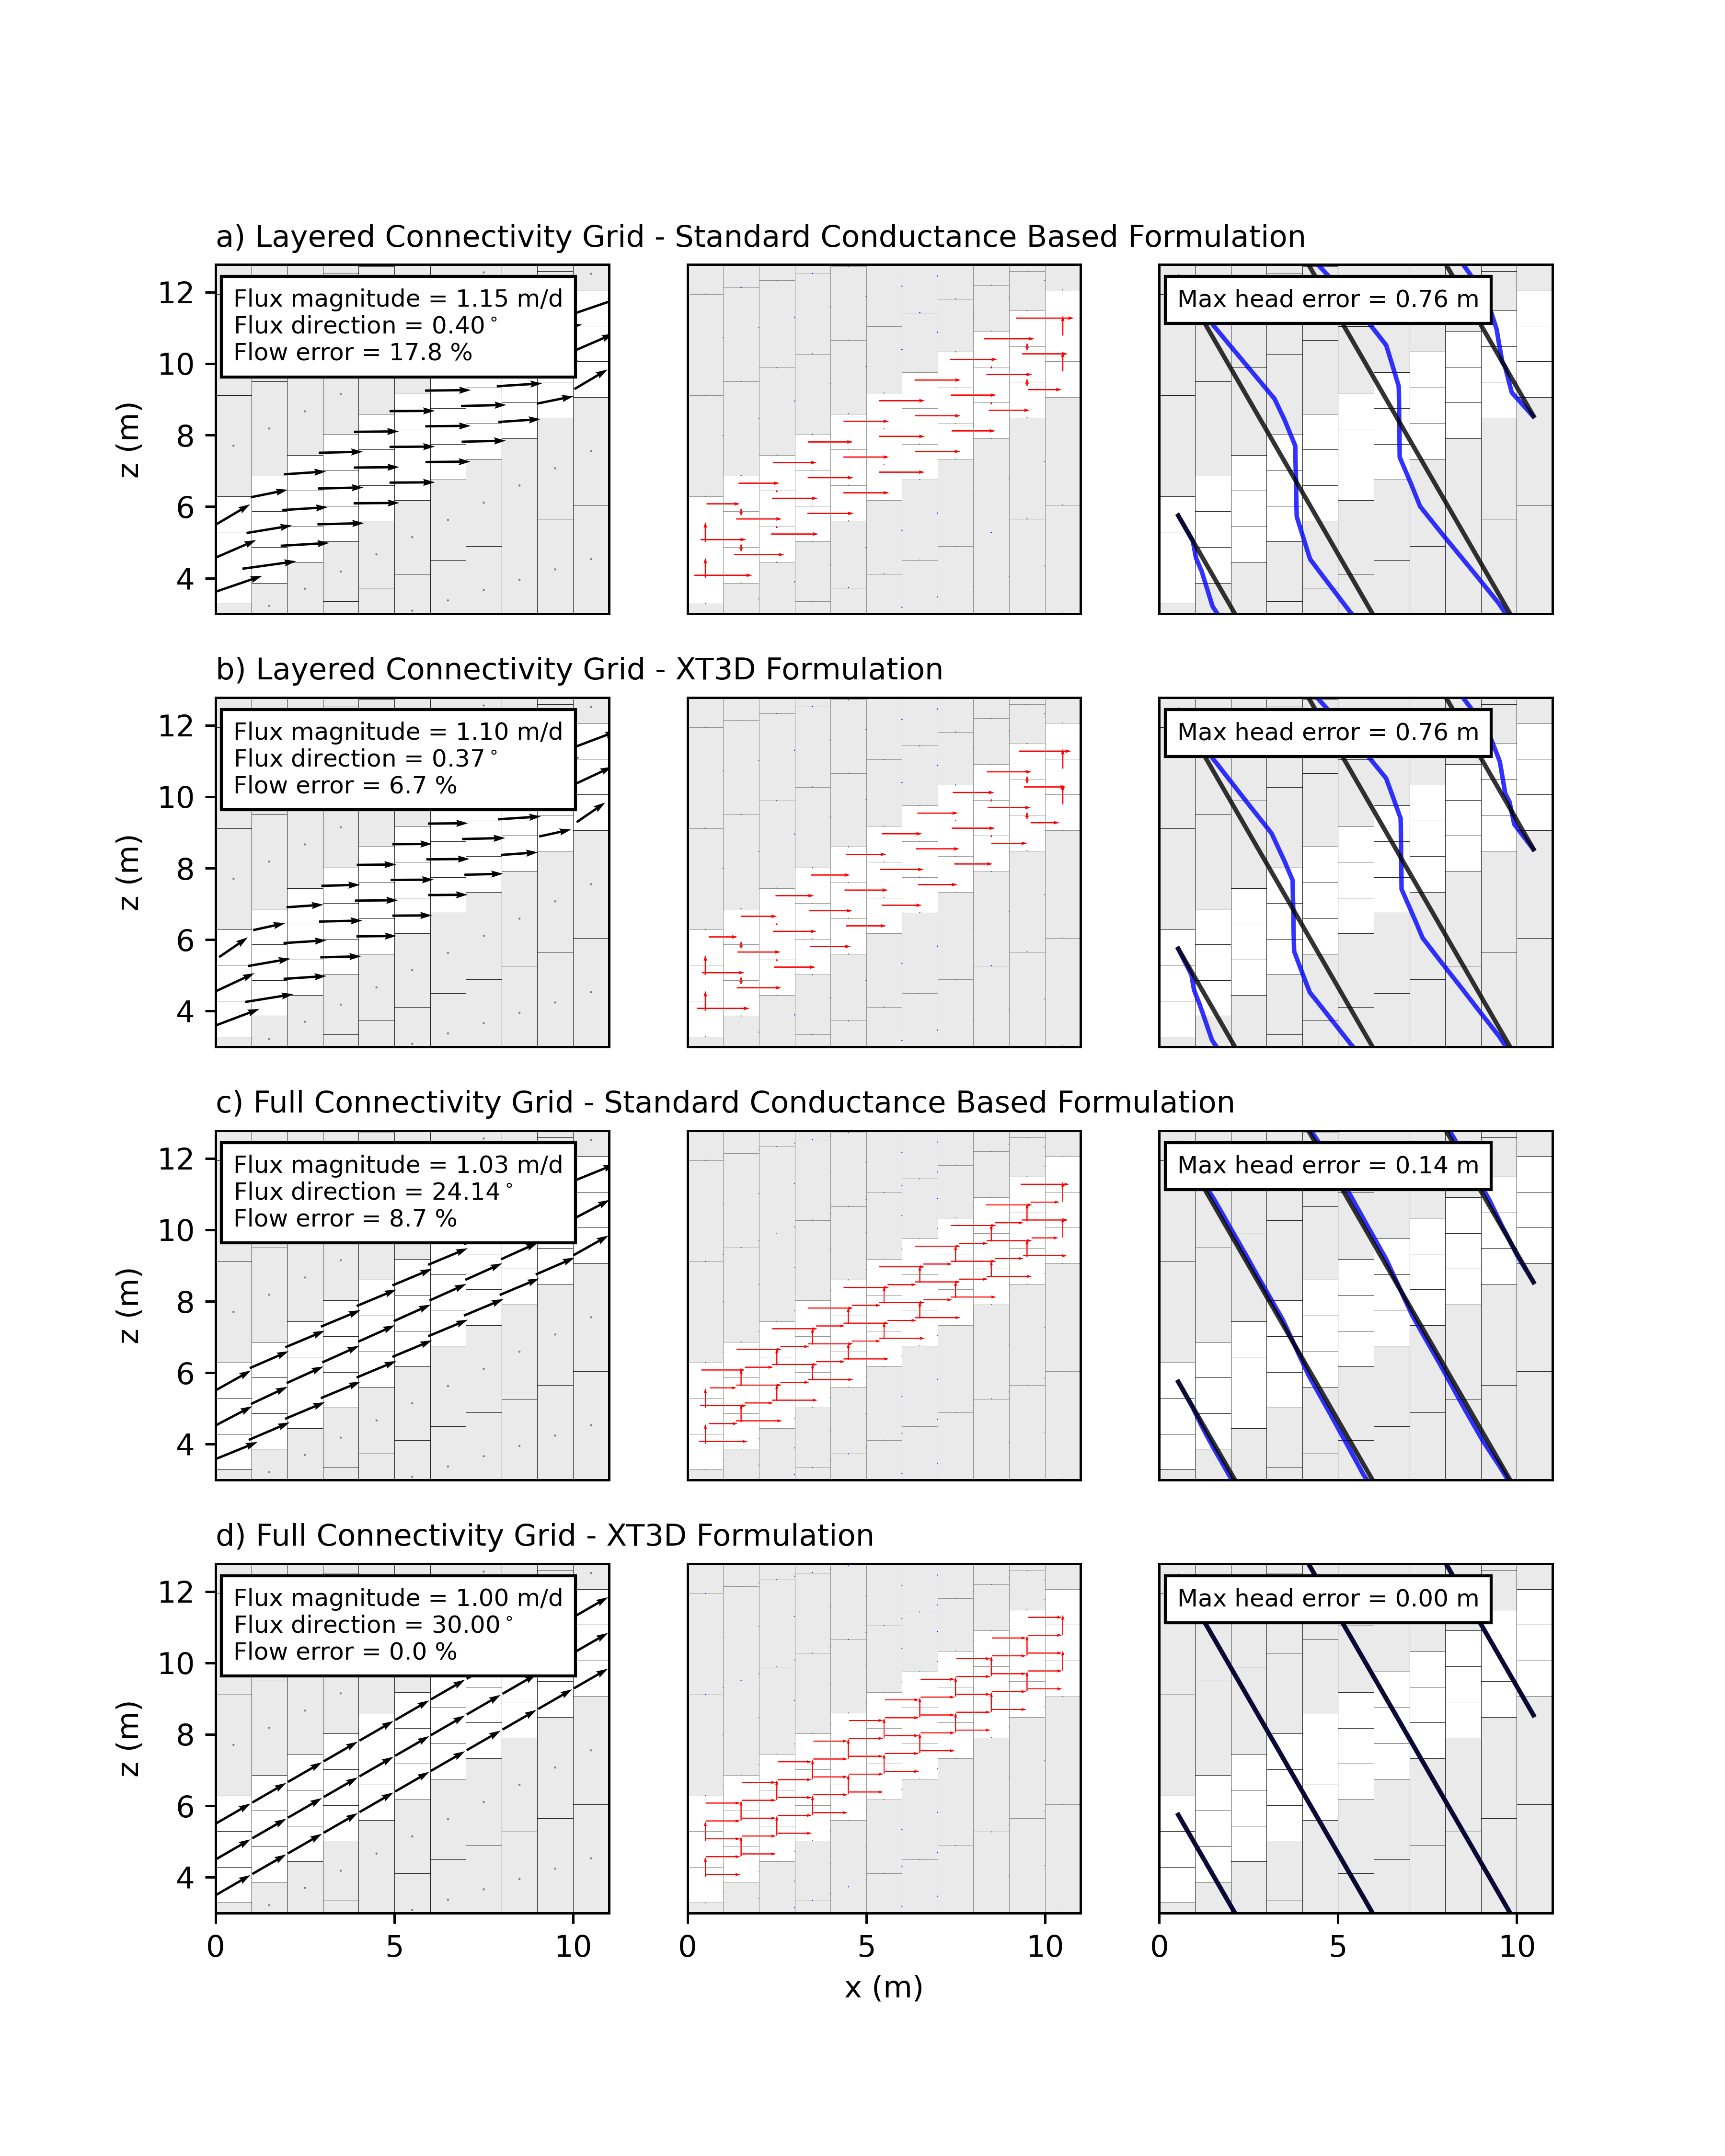
\includegraphics[scale=0.8]{../figures/fig2_paper.png}
	\caption{{\color{red} (CDL: replace ``vertically offset'' with ``layered connectivity'' and ``vertically staggered'' with ``full connectivity''.)} Numerical results for the test problem using base case settings for layered connectivity and full connectivity grids, with the standard conductance based formulation as well as the XT3D formulation. The left panel of each scenario shows the calculated specific discharge at each cell centre (black arrows) with head contours (orange). The right panel shows the face flows (red arrows).}
	\label{fig:fig2}
	\end{center}
\end{figure}

\subsection{Grid Resolution}

{\color{red} Should we also consider the horizontal discretisation too? (CDL: I would say no.  Paper is already getting a bit long.)}

\begin{figure}
	\begin{center}
	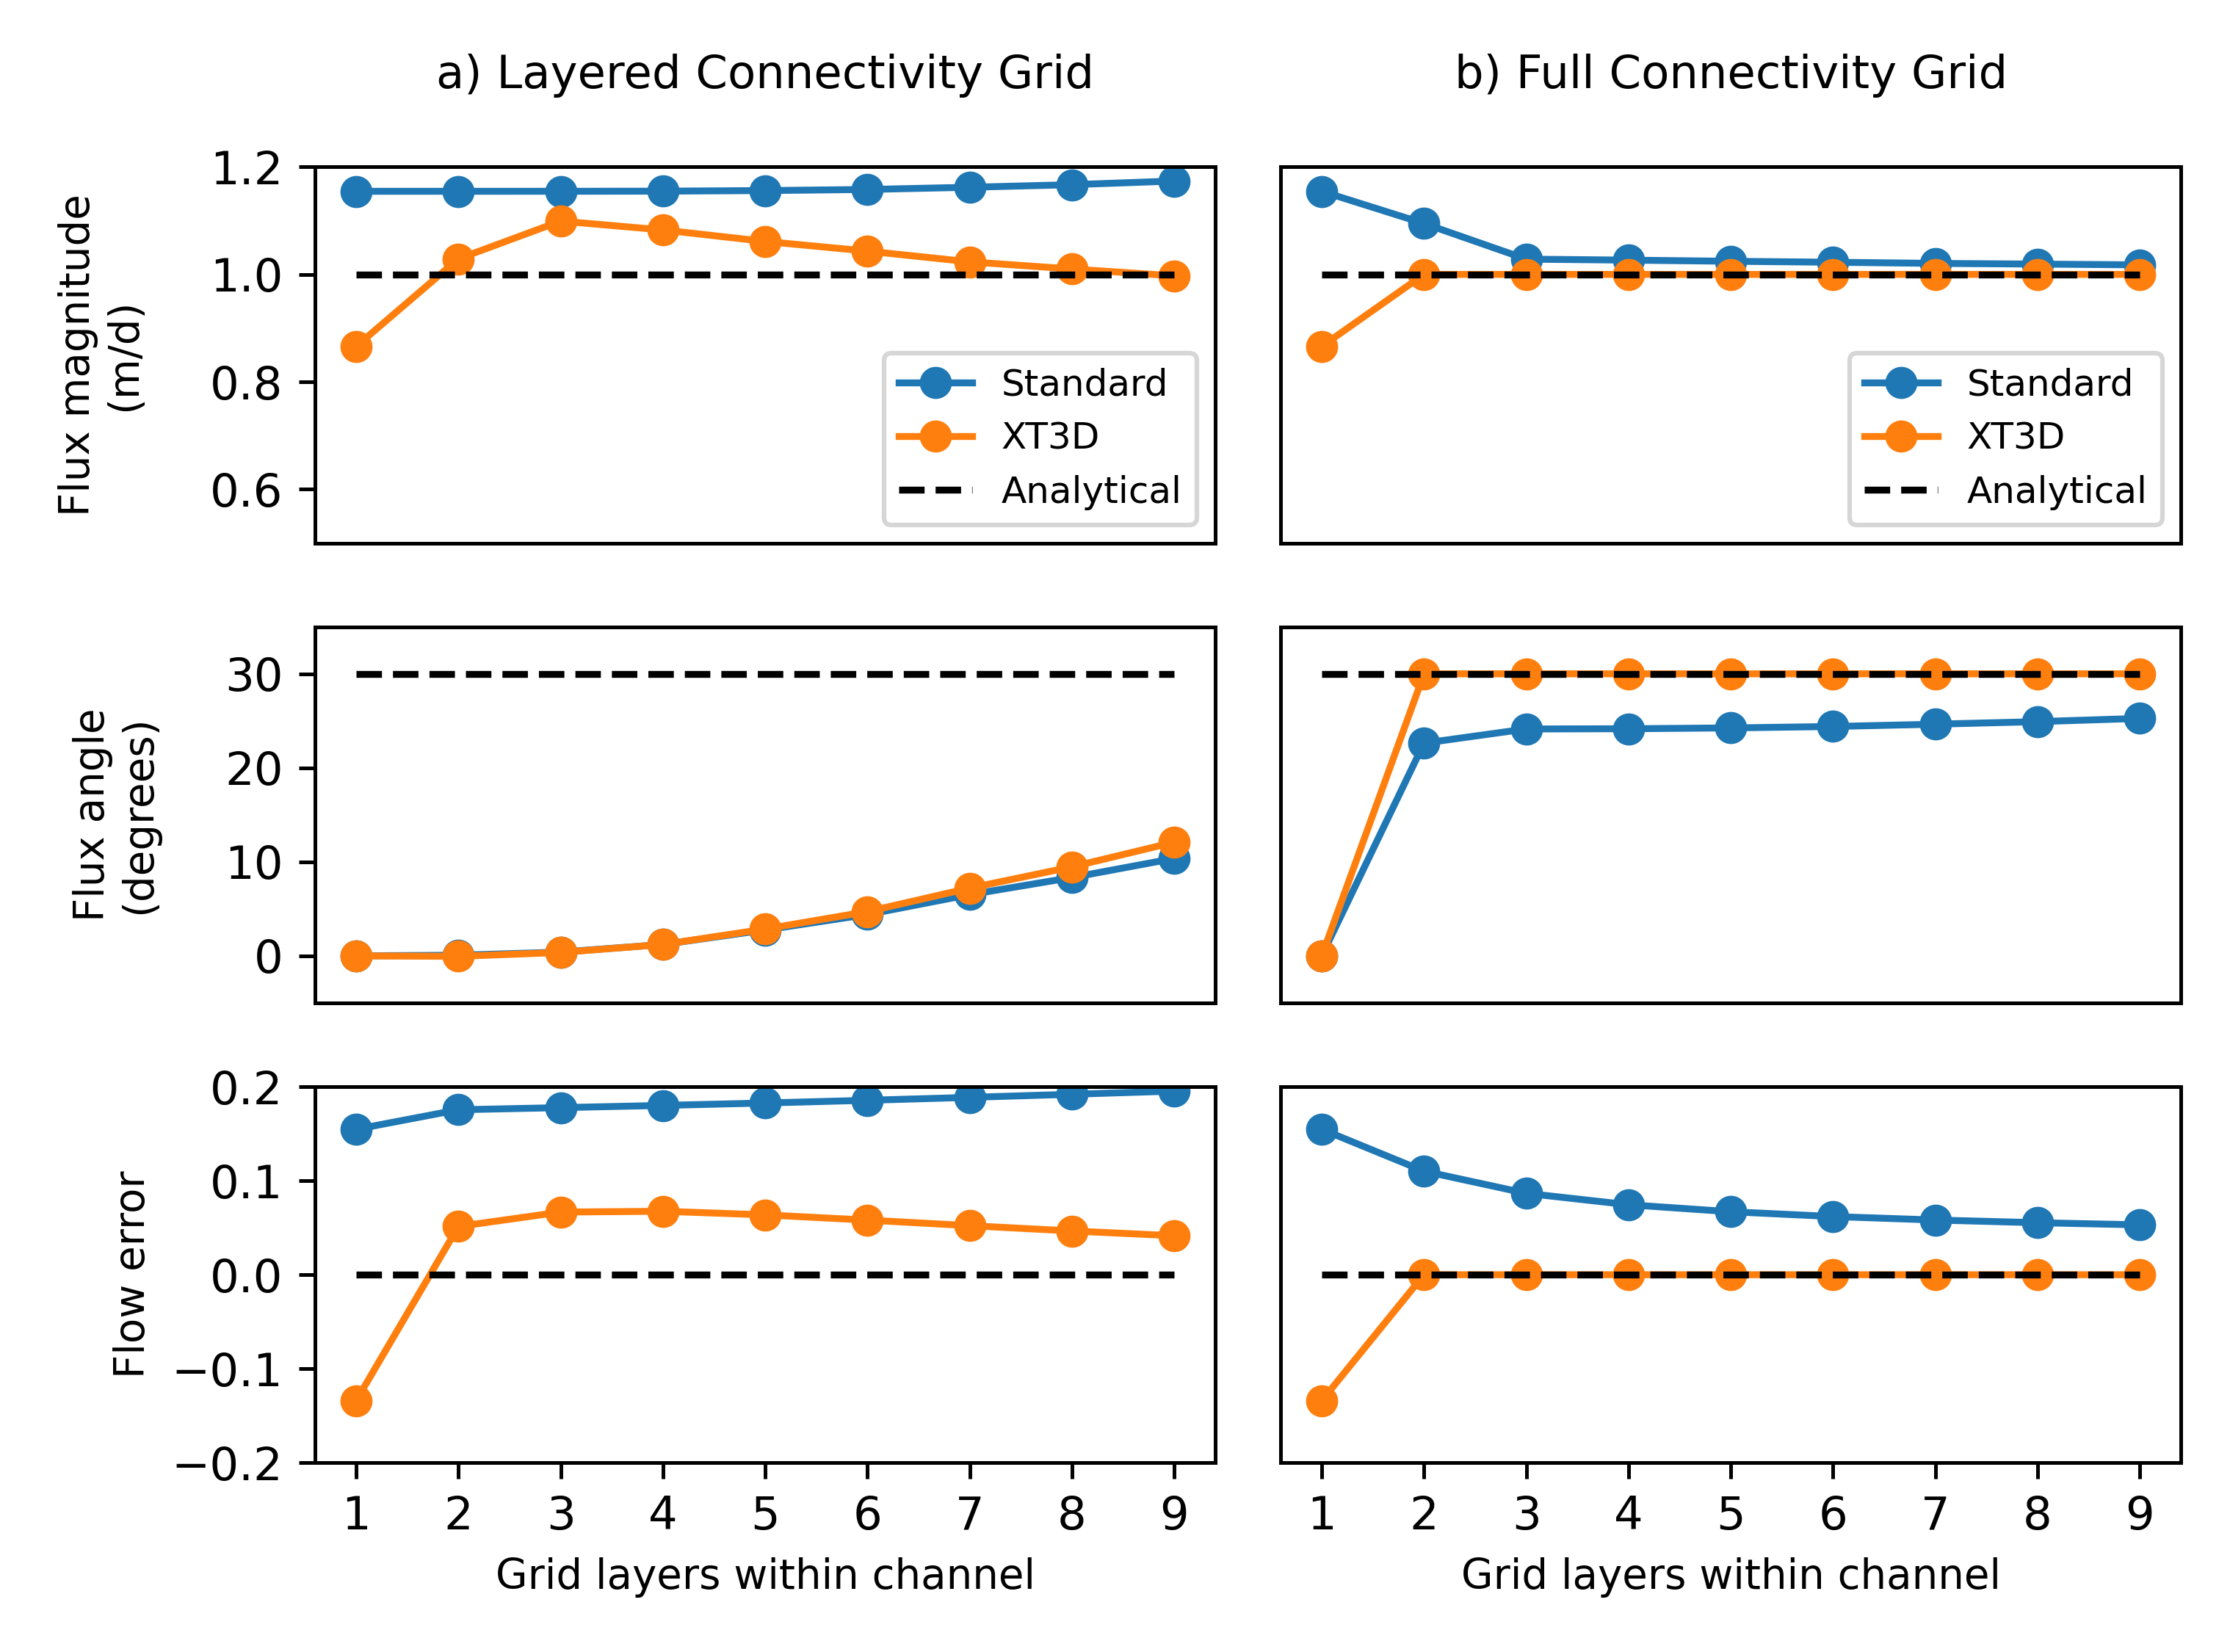
\includegraphics[scale=0.9]{../figures/fig3paper.png}
	\caption{{\color{red} (CDL: replace ``vertically offset'' with ``layered connectivity'' and ``vertically staggered'' with ``full connectivity.'')} Graphs indicating how increasing the number of model layers within a single hydrogeological layer (in this case, the channel) affects (a) flux magnitude of middle cell, (b) flux direction of middle cell and (c) volumetric flow through the channel. We immediately notice the errors layered connectivity grids incur (blue line), and how using a full connectivity grid reproduces the analytical solution from two model layers used to discretise the channel (orange).}
	\label{fig:fig3}
	\end{center}
\end{figure}

The base scenario arbitrarily uses 3 model layers to represent the channel, but it is important to address the question: \emph{How many model layers are required to adequately represent a hydrogeological layer?}. Layered connectivity grids, which have been used by groundwater modellers for decades (ref?) {\color{red} Jim to check, I think there is some refinement guidance for aquitards}, are almost always configured as one model layer per hydrogeological unit. However, although computationally efficient, we investigate the effect of altering resolution within the channel by using the base case and varying number of cells per channel width from one to nine (Figure \ref{fig:fig3}). We compare modeled flux magnitude and direction in the center cell, as well as the volumetric flow against the analytical solution.

Flux magnitude error for layered connectivity grids peaked at around 10\% but improved and tended to zero with refinement. Flux direction for full connectivity grids is clearly a major issue, being reported as horizontal for one model layer per channel width, and only improved to 12$^{\circ}$ for 9 layers per channel width. Flow through the channel peaked at 13\% error but decreased to only a 4\% error for 9 layers per channel width.

The results for the full connectivity grid clearly shows that a minimum of two layers per channel width is required to match the analytical result for flux magnitude, direction and volumetric flow. This is an important finding as it demonstrates that computational efficiency can be made using a full connectivity grid over a rectilinear grid overlay approach, but it is important to use a minimum of two model layers per hydrogeological unit to allow vertical fluxes to be incorporated into the flow solution. 

\subsection{Dip angle and conductivity contrast}

The base case scenario uses a dip angle of 30$^{\circ}$ and an extreme conductivity contrast between channel and domain of $1:10^{-6}$. Here, we investigate the behavior of the flow solution for a wide range of channel inclines by systematically changing the dip angle by 2.5$^{\circ}$ from 0 to 80 $^{\circ}$. Similarly, we examine the solution for multiple conductivity contrasts by changing the domain conductivity to 2, 5, 10 and 100 times less than the channel. Simulated flux magnitude and direction of the centre cell for all combinations are plotted against the analytical solution in Figure \ref{fig:fig4}. 

Traditional layered connectivity grids without XT3D shows rapid diversion of flux magnitude and direction from the analytical solution as dip increases (Figure \ref{fig:fig4a}). Use of the XT3D option keeps the flux magnitude somewhat on-track until about 30 $^{\circ}$ when the solution starts peeling away from the analytical. Flux direction is improved for the homogeneous scenario, but not for the heterogeneous scenarios. The full connectivity grid on the other hand, even without XT3D, roughly follows the analytical solution for flux magnitude and direction until around 65 $^{\circ}$ when it starts to ``fall-apart.'' There are also spikes at certain dip angles which are related to transitions between cell connections due to changing cell face overlaps. The full connectivity grid with XT3D clearly boasts the best results with the flux magnitude and direction matching the analytical until 65 $^{\circ}$, with the exception of a slight decrease in flux direction after 45 $^{\circ}$.

These results confirm that full connectivity grids with XT3D not only outperform the alternatives when modelling dipping hydrogeological unit, but come extremely close to the analytical solution.

\begin{figure}[p!]
\centering
\begin{subfigure}{0.9\textwidth}
	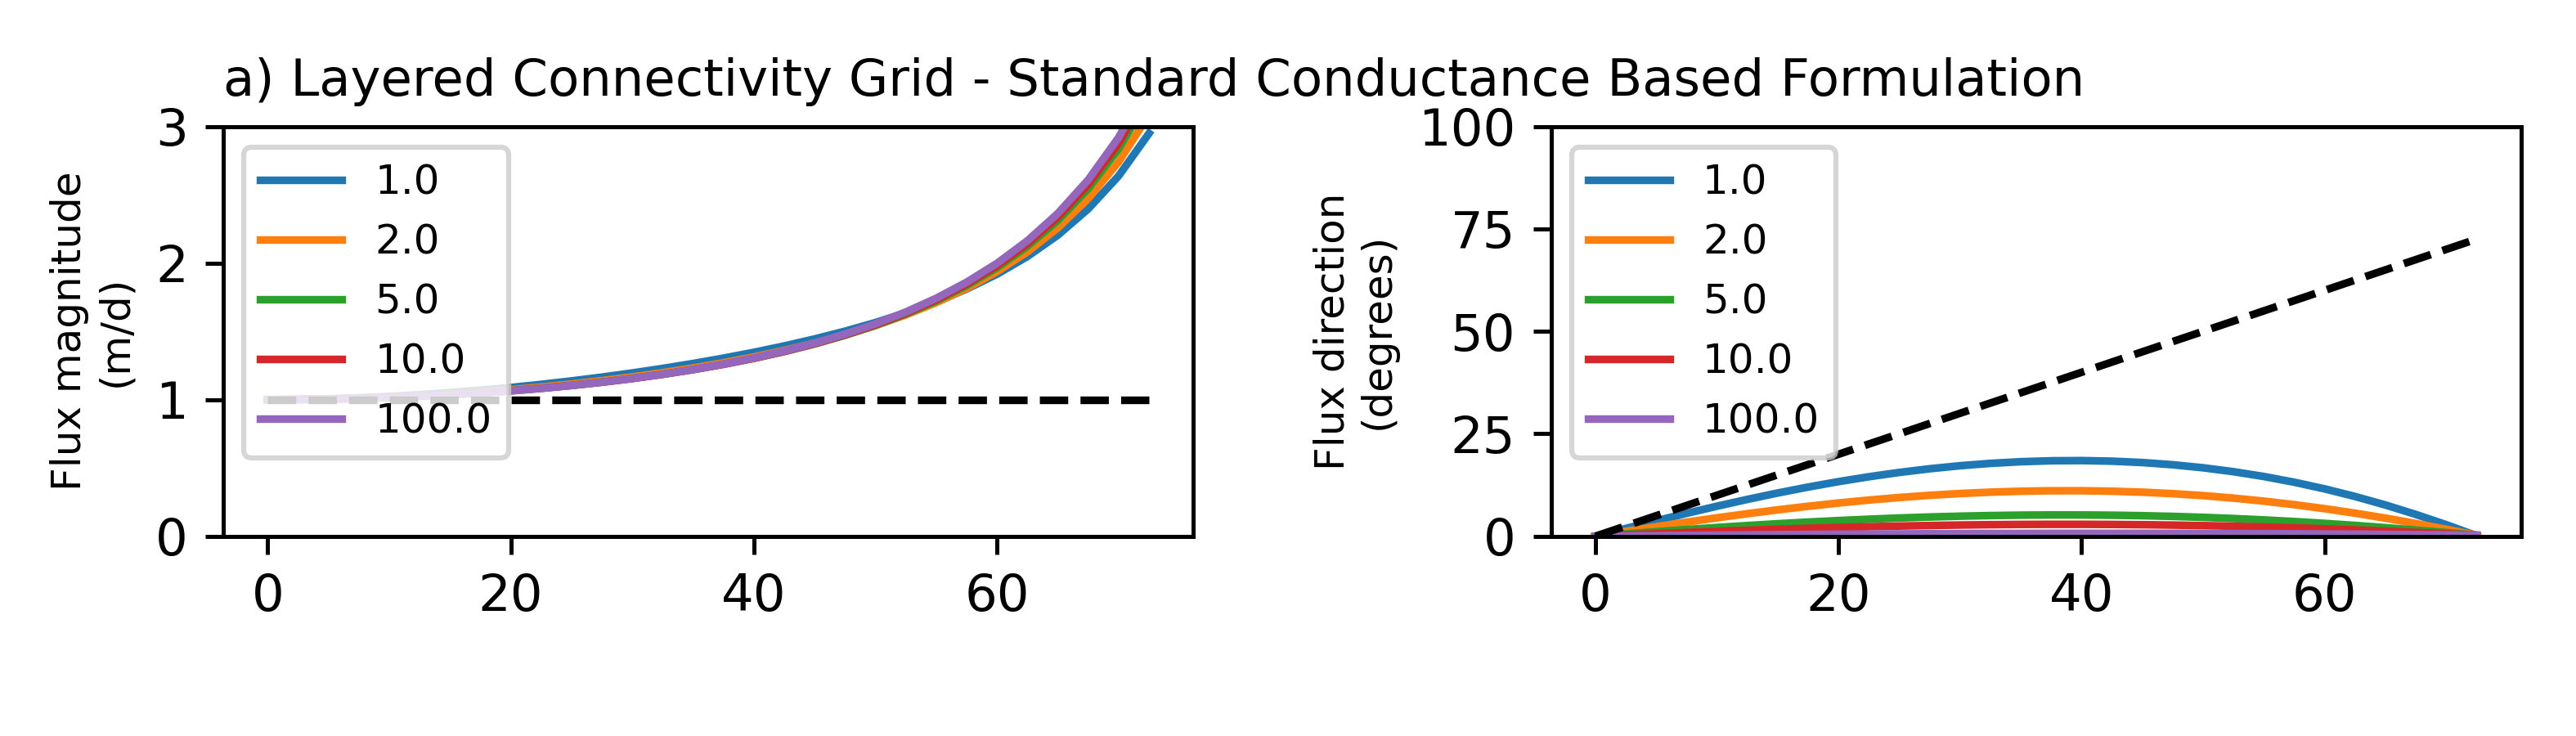
\includegraphics[width=\textwidth]{../figures/fig4_0_paper.png}
	\caption{layered connectivity grid, standard conductance-based formulation}
	\label{fig:fig4a}
\end{subfigure}
\begin{subfigure}{0.9\textwidth}
	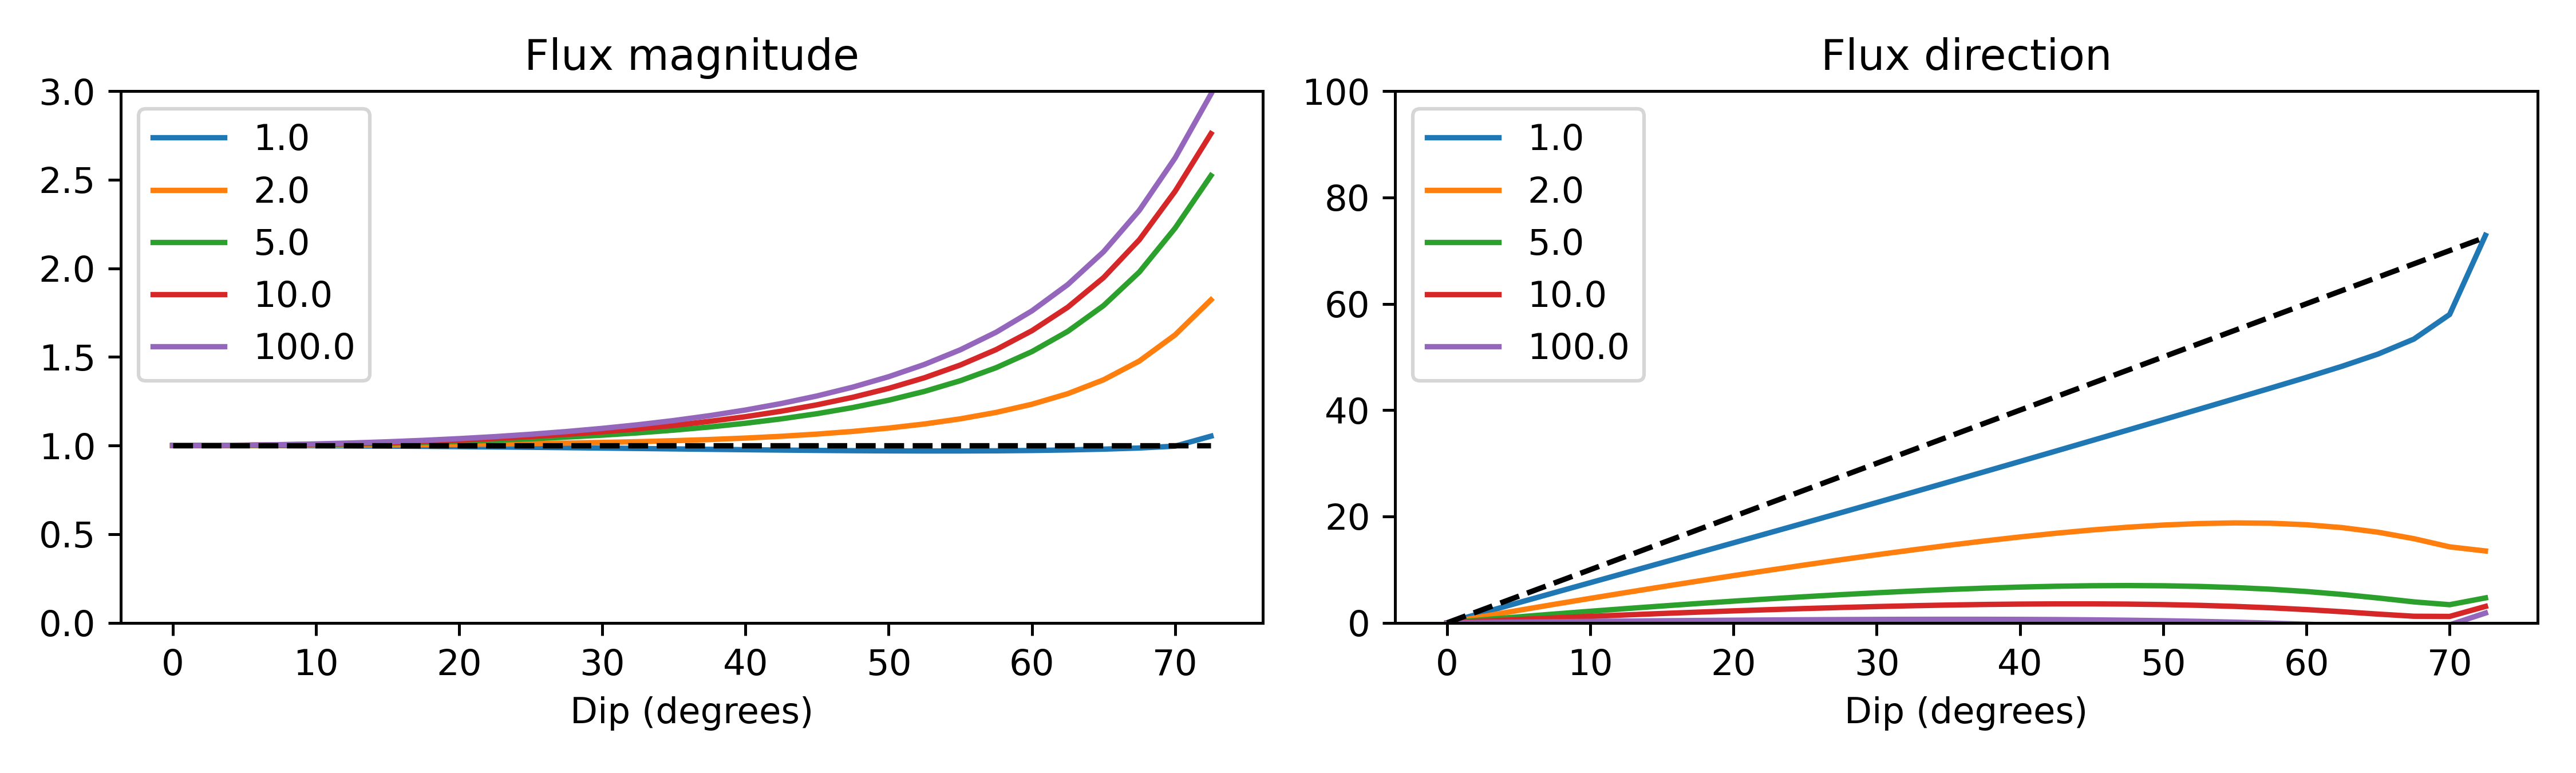
\includegraphics[width=\textwidth]{../figures/fig4_1_paper.png}
	\caption{layered connectivity grid, XT3D}
	\label{fig:fig4b}
\end{subfigure}
\begin{subfigure}{0.9\textwidth}
	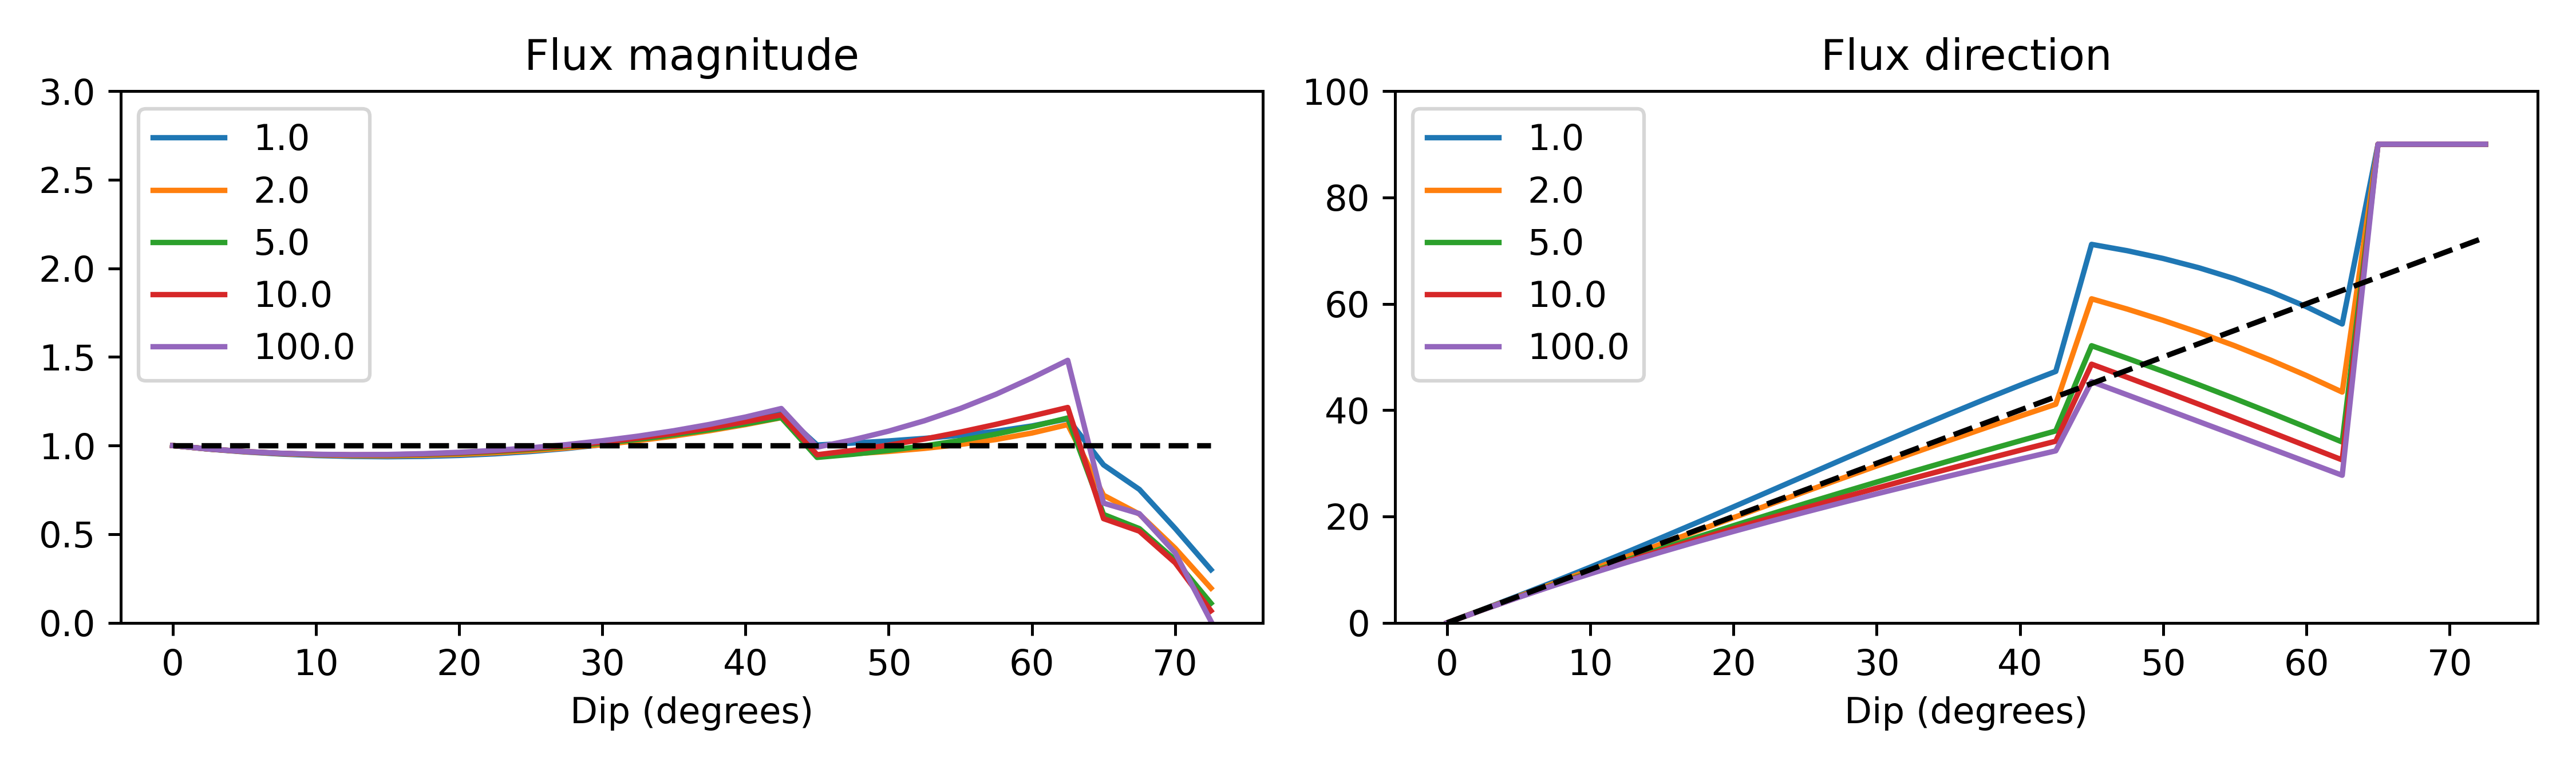
\includegraphics[width=\textwidth]{../figures/fig4_2_paper.png}
	\caption{full connectivity grid, standard conductance-based formulation}
	\label{fig:fig4c}
\end{subfigure}
\begin{subfigure}{0.9\textwidth}
	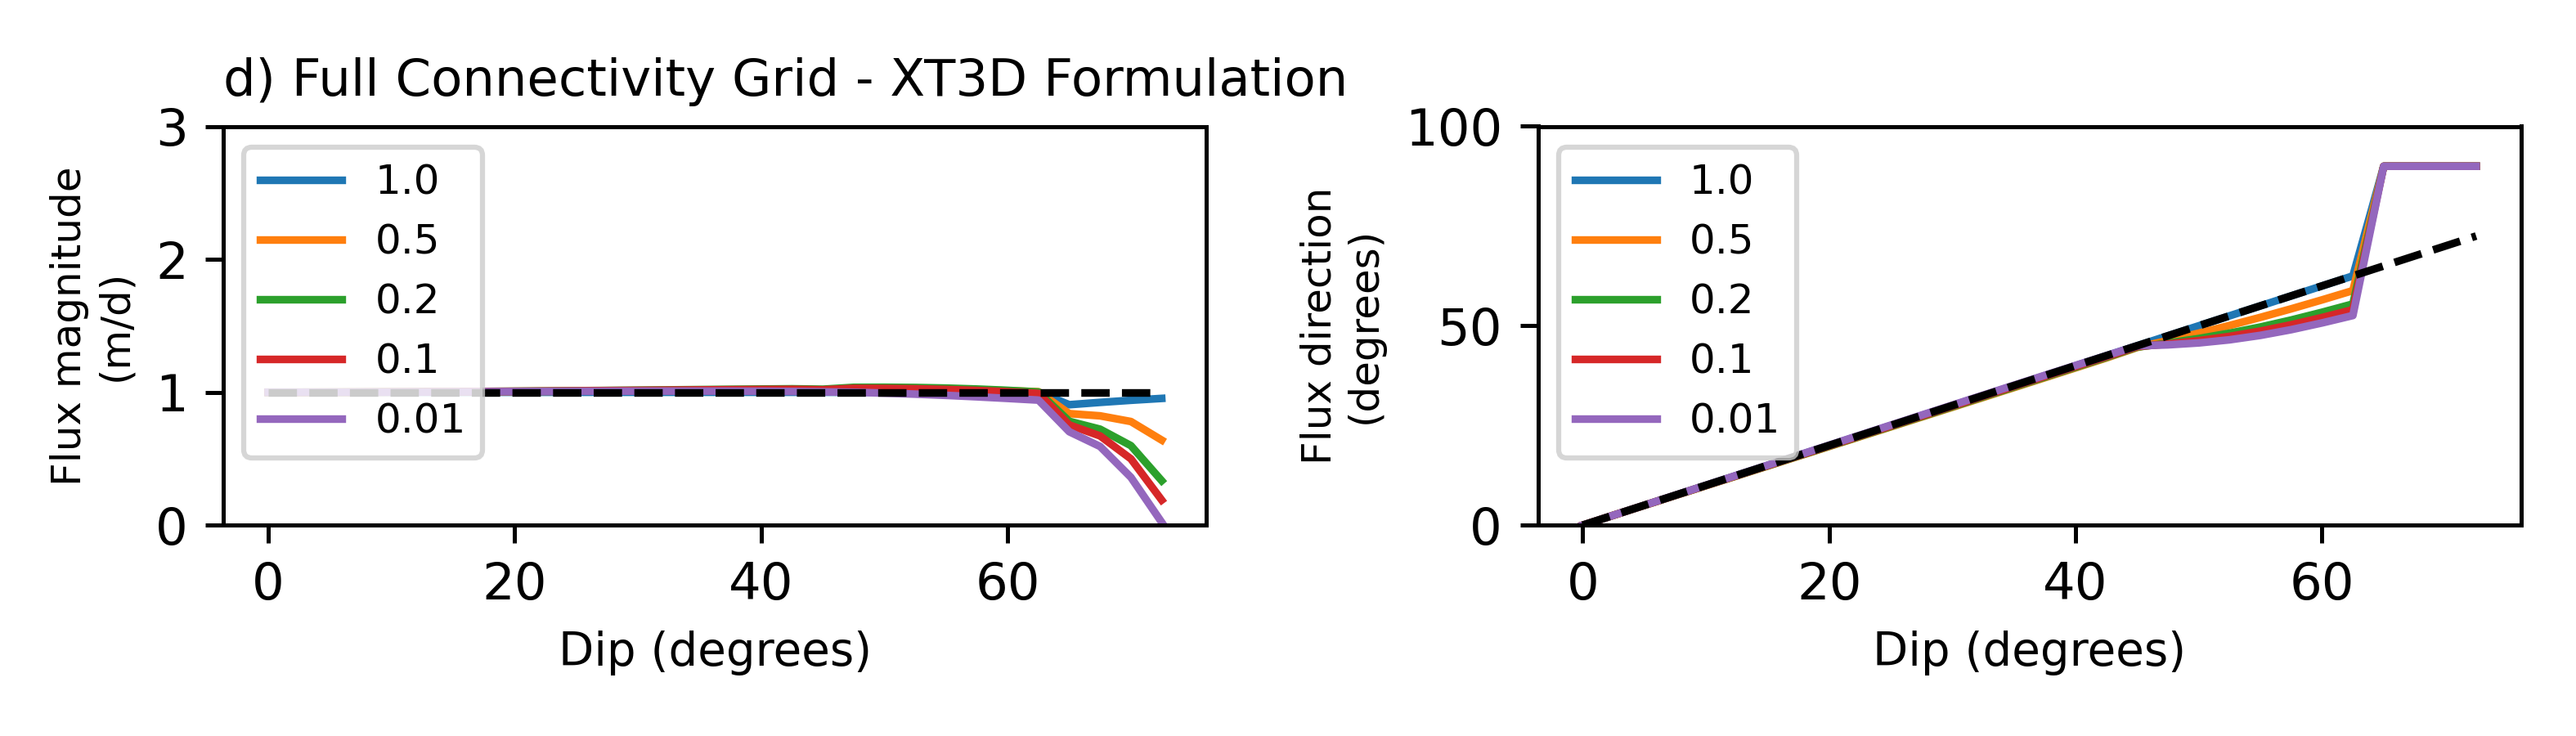
\includegraphics[width=\textwidth]{../figures/fig4_3_paper.png}
	\caption{full connectivity grid, XT3D}
	\label{fig:fig4d}
\end{subfigure}

\caption{{\color{red} (CDL: replace ``vertically offset'' with ``layered connectivity'' and ``vertically staggered'' with ``full connectivity''.)}Flux magnitude and direction for centre cells for varying contrasts in log conductivity (blue, orange, green, red lines) for varying dip angles (x-axis). The analytical value is shown in black dashed line.}
\label{fig:figures}
\end{figure}

\subsection{Anisotropy}

The base case and subsequent scenarios have assumed isotropic conductivity. However, sedimentary layers often exhibit anisotropic conductivity, and therefore we examine the gridding strategies using anisotropic and dipping conductivity tensors, with reduced conductivity perpendicular to the channel by 10, 100, 1000 and 10,000. We also include the isotropic scenario (ratio of 1). Results are presented in Figure \ref{fig:fig5}. 
Layered connectivity grids produce flux magnitude and flow results that significantly deviate from the analytical solution (blue line), whilst full connectivity grids reproduce the analytical solution (orange line). These results verify, once again, our proposed method of using full connectivity grids to model dipping anisotropic layers.


\begin{figure}
	\begin{center}
	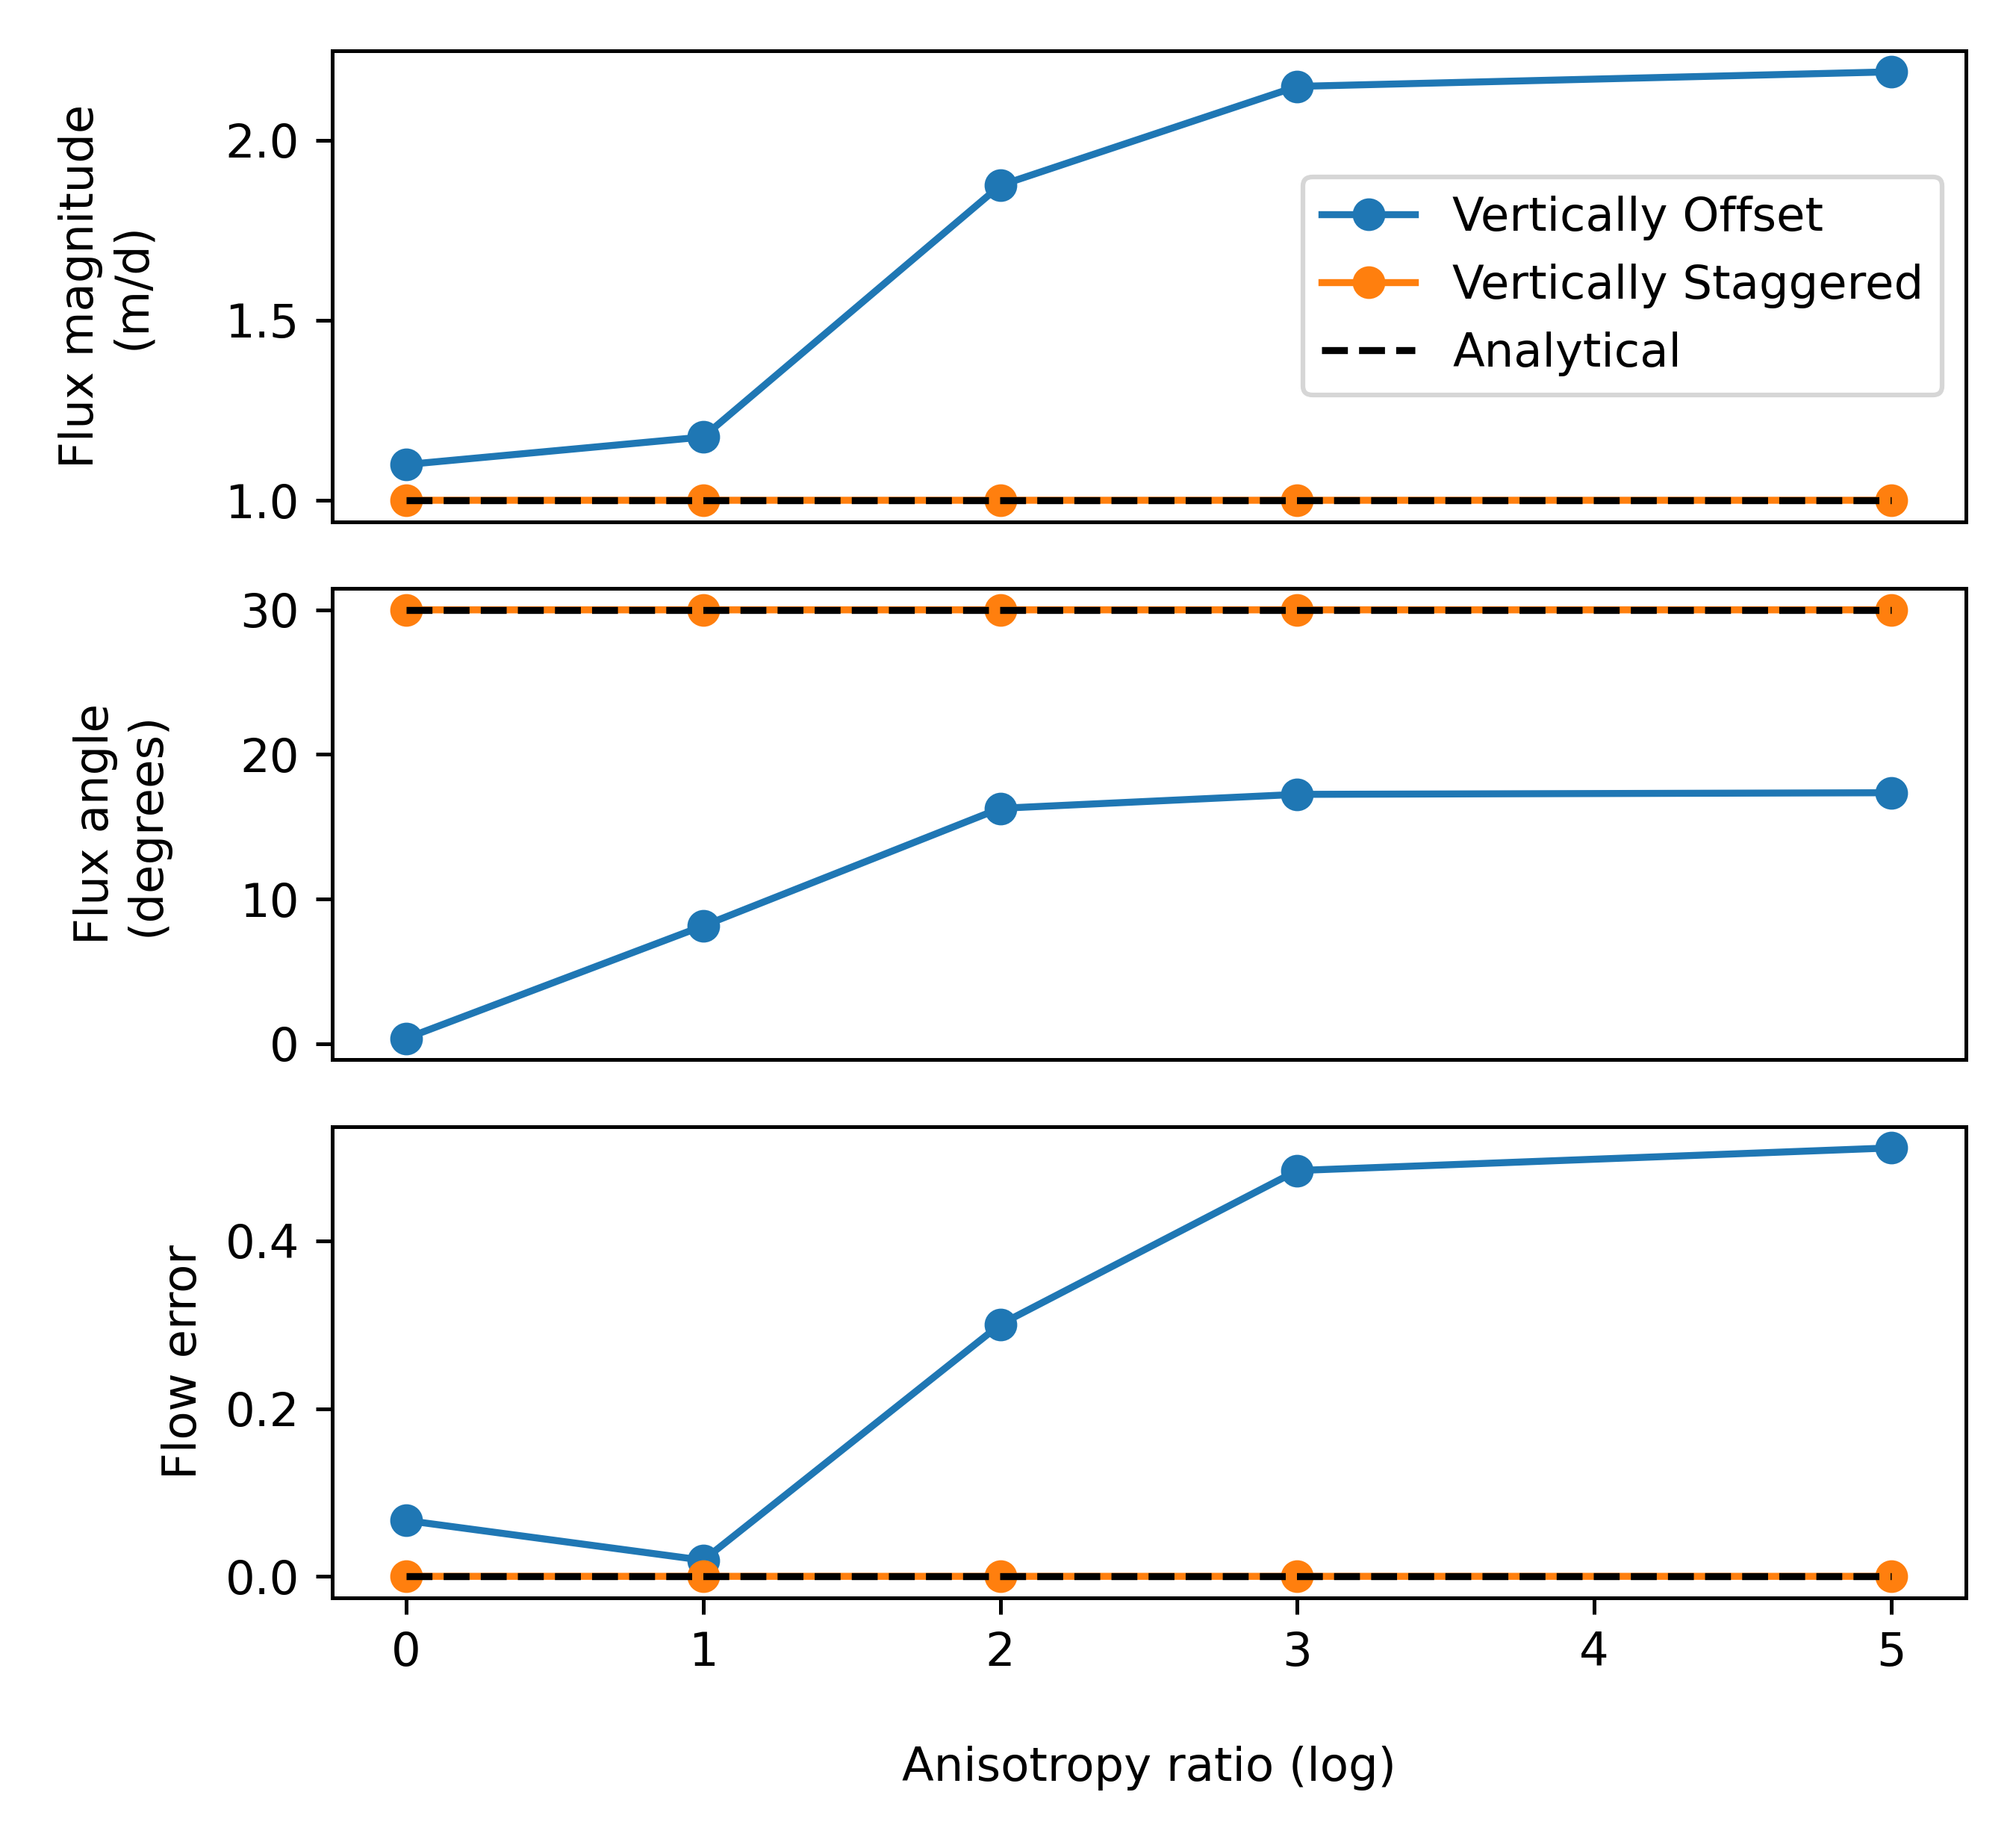
\includegraphics[scale=0.9]{../figures/fig5paper.png}
	\caption{Varying anisotropy ratios of conductivity withing the channel and the resulting (a) flux magnitude of middle cell, (b) flux direction of middle cell and (c) volumetric flow through the channel. }
	\label{fig:fig5}
	\end{center}
\end{figure}


\section{Conclusions}

 {\color{red} CDL: I added the following two paragraphs in an attempt to summarize my understanding of the main conclusion.  Feel free to edit or scrap as you see fit.}

\cite{bardot2022} revisited the capability of MODFLOW to accurately simulate groundwater flow through sedimentary structures.  They concluded that the XT3D multi-point flux approximation in MODFLOW 6 significantly improves the accuracy of simulated flows for rectilinear grid overlay approaches in which locations of sedimentary structures are mapped onto a relatively fine model grid.  They also concluded that the XT3D multi-point flux approximation did not perform as well as anticipated for vertically offset grids, which are advantageous for significantly reducing the number of layers required for many problems.  They hypothesized that the inherent connectivity in DIS and DISV layered grids in MODFLOW 6 was inadequate for allowing the XT3D multi-point flux approximation to work as intended.

In this paper, we confirm that the layered connectivity implemented in DIS and DISV model grids is inadequate for simulating groundwater flow through steeply dipping sedimentary structures, even when the XT3D multi-point flux approximation is used.  However, when additional cross connections are added to comprise a grid with full connectivity, there is a substantial increase in the accuracy of simulated flows.  Importantly, this accuracy improvement requires that at least two model layers are used to represent the steeply dipping sedimentary structure.  The primary conclusion of this paper, therefore, is that that the XT3D multi-point flux approximation implemented in MODFLOW 6 can be combined with vertically offset grids to efficiently and accurately model flows through sedimentary structures.  Prior to this work, the capability to efficiently and accurately model flow through sedimentary structures was generally restricted to finite element simulators.

This paper presents a solution for accurately representing steeply dipping flow structures groundwater utilising MODFLOW 6. \citep{bardot2022} demonstrated that the flux magnitude in highly dipping scenarios was erroneous when utilising layered connectivity grids.  {\color{red} CDL: Also applicable for MODFLOW-USG DISU grids.} More significantly, the direction of fluxes were inaccurate, neglecting the vertical component of the flux. The issues observed in the existing study of \citep{bardot2022} partially related to the implementation of only within-layer horizontally connections, limiting the model capacity to simulate the vertical component of the flow. The present study developed an approach which utilised full connectivity grids \cite{modflow6gwf} to overcome the perceived problems. Through comparison of the previous layered connectivity and proposed full connectivity approached to the analytical solution presented in \citep{bardot2022}, we demonstrate that the use of full connectivity grids (in conjunction with the XT3D formulation) is an accurate method to simulate flow through dipping hydrogeological layers. However, accurate representation of flows requires a minimum of two model layers per hydro geological unit to allow for vertical connections to induce flows. 

Points:

1) Furthermore, we point out the nuances in specific discharge calculations and the ambiguity introduced when assessing model behaviour.  MODPATH and MT3D

2) The concepts in this paper have been easiest to discuss in terms of grid layers, but they're not limited to layered grids.

3) (Random thought) The use of full connectivity grids improved the accuracy of the transect solutions; however, the results of \citep{bardot2022} using unstructured meshes that conformed to the channel geometry preformed better in isotropic grids. If you force the normal flux to be the same at the interface of the domain and channel, the analytical solution would suggest a uniform gradient either side, do we introduce an error if the faces don't align with the channel correctly?  Would figure 2 show a correction for this if the anisotropic scenario was tested?

 {\color{red} CDL: Maybe worthwhile to implement full connectivity approaches for DIS and DISV grids in mf6.}

\section{Acknowledgments}
We would like to acknowledge....

\section{Supporting Information}

\section{Appendix}

\bibliography{references.bib}


\end{document}
